\documentclass[tikz=true]{standalone}
\usepackage{graphicx, standalone}
\usepackage[compat=1.1.0]{tikz-feynman}
\usepackage{tikz}
\usepackage{amsmath, amssymb}
\usepackage{euler}
\usepackage{fontspec}
\setmainfont{MinionPro}

\renewcommand{\k}{\ensuremath\text{k}}
\newcommand{\kp}{\ensuremath\text{k}'}
\newcommand{\q}{\ensuremath\text{q}}

\begin{document}

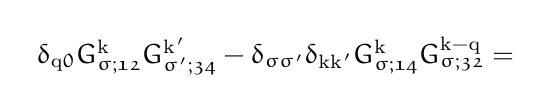
\begin{tikzpicture}[baseline=(current bounding box.center)]
    \node {$\delta_{\q0}G_{\sigma;\mathfrak{12}}^{\k}G_{\sigma';\mathfrak{34}}^{\kp}-\delta_{\sigma\sigma'}\delta_{\k\kp}G_{\sigma;\mathfrak{14}}^{\k}G_{\sigma;\mathfrak{32}}^{\k-\q}=$};
\end{tikzpicture}
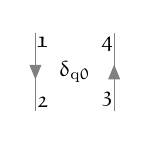
\begin{tikzpicture}[baseline=(current bounding box.center)]
	\begin{feynman}[small]
		\vertex (a1);
		\vertex[below=of a1] (a2);
		\vertex[right=of a1] (b1);
		\vertex[below=of b1] (b2);
		
		\def\sc{0.8};
		
		\node[below right=-0.2em and -0.3em of a1] {\scalebox{\sc}{$\mathfrak{1}$}};
		\node[above right=-0.2em and -0.3em of a2] {\scalebox{\sc}{$\mathfrak{2}$}};
		\node[below left=-0.2em and -0.3em of b1] {\scalebox{\sc}{$\mathfrak{4}$}};
		\node[above left=-0.2em and -0.3em of b2] {\scalebox{\sc}{$\mathfrak{3}$}};
		
		\node (content) at ($(a1)!0.5!(b2)$) {\scalebox{\sc}{$\delta_{\q0}$}};
		
		\diagram* {
			(a1) -- [fermion, gray] (a2),
			(b2) -- [fermion, gray] (b1)
		};	
	\end{feynman}
\end{tikzpicture}
\begin{tikzpicture}[baseline=(current bounding box.center)]
	\node {$-$};
\end{tikzpicture}
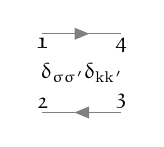
\begin{tikzpicture}[baseline=(current bounding box.center)]
	\begin{feynman}[small]
		\vertex (a1);
		\vertex[below=of a1] (a2);
		\vertex[right=of a1] (b1);
		\vertex[below=of b1] (b2);
		
		\def\sc{0.8};
		
		\node[below=-0.2em of a1] {\scalebox{\sc}{$\mathfrak{1}$}};
		\node[above=-0.2em of a2] {\scalebox{\sc}{$\mathfrak{2}$}};
		\node[below=-0.2em of b1] {\scalebox{\sc}{$\mathfrak{4}$}};
		\node[above=-0.2em of b2] {\scalebox{\sc}{$\mathfrak{3}$}};
		
		\node (content) at ($(a1)!0.5!(b2)$) {\scalebox{\sc}{$\delta_{\sigma\sigma'}\delta_{\k\kp}$}};
		
		\diagram* {
			(a1) -- [fermion, gray] (b1),
			(b2) -- [fermion, gray] (a2)
		};	
	\end{feynman}
\end{tikzpicture}

\end{document}